\section{开发者激励模型}
开发者激励协议,DIP,包括两个环节:DApp评分以及开发者激励分配。

首先对于构建一个优秀的排名系统,其意义在于为第三方开发者提供了方便且高效的应用推广平台,同时也能为用户提供可信的推荐环境。正如目前移动端的App Store平台,优秀App在排行榜上拥有更显著的位置进而能受到更多用户的关注,而用户能通过排行榜上直接获取高质量的App无疑能提高其体验。更进一步地,App排名也可以应用于关键词搜索中,类似于搜索引擎和电商平台中的搜索功能,与关键词相关的候选DApp将按排名分顺序展示在搜索结果中,增加用户对搜索结果的满意程度。

另一方面,正如我们在第~\ref{sec:back_ground}章所提到的,DIP旨在为优秀DApp的开发者提供奖励,这进一步增加了开发者设计优秀DApp的动机,对整个生态的开发起到了促进作用。因此DIP第二个环节则是根据DApp评分排名提出公平的奖励分配机制。

\subsection{模型表示}
\label{subsection:parameters}
首先我们给出DIP模型中涉及的符号表示。
\begin{itemize}
	\item $\mathcal{A}=\{a_1,a_2,...,a_m\}$表示一定时间内所有参与评选的投票用户的集合,注意的是只有在一定时间内调用过任何DApp的外部账户(External Owned Account)才会被定义为投票用户。同时期所有用户集合表示为$$\mathcal{A}^*=\{a_1,a_2,...,a_m,a_{m+1},...,a_{m^*}\}$$,即有$m^*-m$个用户没有调用任何智能合约。
	\item $\mathcal{D}=\{d_1,...,d_n\}$表示一定时间内所有DApp的集合。
	\item $e_{ij},i=1,2,...,m, j=1,2,...,n$表示在一定时间内用户$a_i$对DApp $d_j$的总调用次数。鉴于区块链系统所具有的公开性,去中心化等特性,因此DIP评分模型和传统中心化的应用商城评分系统有所不同。简单地说,DIP在去中心化环境中基于用户调用行为对DApp进行评分,具体描述见下一节。
	\item $\nr_i, i=1,2,...,m$表示参与评选的用户$a_i$在一定时间内投票效用。~\cite{Nebulasyellowpaper}中已经证明NR值是衡量一个用户的有效价值尺度,故我们也把其用作DIP模型中用于决定用户投票效用的重要指标。
	\item $\nr_{ij}, i=1,2,...,m,j=1,2,...,n$表示用户$a_i$对DApp $d_j$的分贡献值。可以理解为$a_i$愿意为$d_j$投的票数。%在我们的模型里由$a_i$对所有DApp的调用次数决定。
	\item $S_j, j=1,2,...,n$,表示DApp $d_j$的排名分,由该DApp从用户获得的所有分贡献值决定。直观地,排名分的高低直接决定了DApp在排行榜上所处的位置。%一种对排名分最简单的定义方式为所有分贡献值相加。而我们的模型采取了更合理的排名分计算方式。
	\item $M$表示星云团队用于给与开发者奖励总奖金池。实际发放的奖励总额会根据该阶段社区参与度来适当进行加权调整。
	\item $U_j, j=1,2,...,n$,表示DApp $d_j$开发者最终获得的奖励,这个奖励由奖励总额以及所有DApp的排名分共同决定。%生活中常见的评奖方式通常具有凹函数性质,例如第一名10000元,第二名5000元,第三名2000元。我们的奖励函数具有同样性质且具有更高的可扩展性。
\end{itemize}

\begin{figure}
	\centering
 %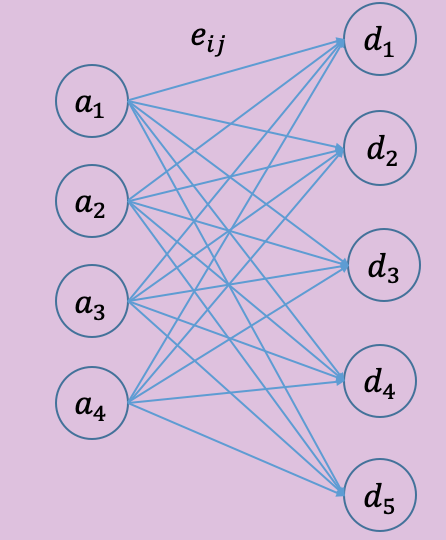
\includegraphics[width = 0.4\textwidth]{../common/m2.png}
  \begin{tikzpicture}
\pgfmathsetmacro{\XTD}{3.8}
\pgfmathsetmacro{\YTD}{1.2}

\tikzset{
  node/.style={draw, circle, on grid, align=center, minimum height=2ex},
}

\node[node] (d1) at (\XTD, 2*\YTD) {$d_1$};
\node[node] (d2) at (\XTD, \YTD) {$d_2$};
\node[node] (d3) at (\XTD, 0) {$d_3$};
\node[node] (d4) at (\XTD, -1*\YTD) {$d_4$};
\node[node] (d5) at (\XTD, -2*\YTD) {$d_5$};

\node [right=0.05 of d1] {${S}_{1}$};
\node [right=0.05 of d2] {${S}_{2}$};
\node [right=0.05 of d3] {${S}_{3}$};
\node [right=0.05 of d4] {${S}_{4}$};
\node [right=0.05 of d5] {${S}_{5}$};

\node[node] (a1) at (-\XTD, 1.5*\YTD) {$a_1$};
\node[node] (a2) at (-\XTD, 0.5*\YTD) {$a_2$};
\node[node] (a3) at (-\XTD, -0.5*\YTD) {$a_3$};
\node[node] (a4) at (-\XTD, -1.5*\YTD) {$a_4$};

\node [left=0.05 of a1] {${\nr}_{1}$};
\node [left=0.05 of a2] {${\nr}_{2}$};
\node [left=0.05 of a3] {${\nr}_{3}$};
\node [left=0.05 of a4] {${\nr}_{4}$};

\draw[->, >=stealth'] (a1) to (d1);
\draw[->, >=stealth'] (a1) to (d2);
\draw[->, >=stealth'] (a1) to (d3);
\draw[->, >=stealth'] (a1) to (d4);
\draw[->, >=stealth'] (a1) to (d5);

\draw[->, >=stealth'] (a2) to (d1);
\draw[->, >=stealth'] (a2) to (d2);
\draw[->, >=stealth'] (a2) to (d3);
\draw[->, >=stealth'] (a2) to (d4);
\draw[->, >=stealth'] (a2) to (d5);

\draw[->, >=stealth'] (a3) to (d1);
\draw[->, >=stealth'] (a3) to (d2);
\draw[->, >=stealth'] (a3) to (d3);
\draw[->, >=stealth'] (a3) to (d4);
\draw[->, >=stealth'] (a3) to (d5);

\draw[->, >=stealth'] (a4) to (d1);
\draw[->, >=stealth'] (a4) to (d2);
\draw[->, >=stealth'] (a4) to (d3);
\draw[->, >=stealth'] (a4) to (d4);
\draw[->, >=stealth'] (a4) to (d5);

\node at (0, 2*\YTD) {$e_{ij}$};

\end{tikzpicture}

\caption{用户与DApp间的交互 \label{fig:interact}}
\end{figure}

综上,用户和DApp之间的交互可以用图~\ref{fig:interact}中的二分图来表示。

\subsection{投票行为}
\label{subsection:voting}
在中心化的App Store\footnote{\url{https://en.wikipedia.org/wiki/App\_store}}中,系统会记录App的下载量等信息,后者也是应用评分的主要参考因素之一。而在区块链场景下,用户对于应用的使用会直接反应在调用合约地址行为上,例如表现为一段时间内用户$a_i$对DApp $d_j$的总调用次数$e_{ij}$。DIP通过用户调用行为作为用户的投票数据来源,相比传统的下载量信息具有如下优点:
\begin{itemize}
	\item 用户调用智能合约行为记录在链上,很难篡改,相比中心化的下载量统计方式更加公开透明;
	\item 调用次数相比下载量信息更加细粒度,下载量只能记录用户一次性行为,而优秀的DApp应具有用户黏性,因此调用次数更能反映用户的真实使用情况。
\end{itemize}

实际上用户在调用智能合约时,还有其他信息可获取,例如调用智能合约过程中的gas消耗以及在调用过程中可能涉及到的资金交互,而DIP没有采取上述两者作为参考依据。

首先,用户每次调用智能合约gas消耗量是与智能合约内部的执行语句相关,而后者与DApp本身质量没有任何相关性。同时,目前星云系统中智能合约调用gas消耗开销平均只有$10^{-8}$数量级的NAS,可以忽略不计。

%所花费的gas费用以及向合约地址支付的费用不会被排名算法考虑进去,即用户支付更多的钱无法提高其投票效用。前者是因为在

而不考虑调用合约过程中资金转移的原因在于有效防作弊手段的缺失。直觉上来说,用户在使用DApp过程中愿意额外支付token确实能提高该DApp的被认同度。但实际情况下,这笔交易中token的最终流向存在以下三种可能。
\begin{enumerate}
\item Token最终归智能合约即DApp开发者所有。这种情况可以认为用户自愿付出这些钱给DApp,但此时DApp开发者相当于已经从中获益,再提高其排名获取额外奖励的意义不大。

\item DApp机制设计需要资金流通,例如博彩类DApp,其与用户之间存在大量资金交互。这是一种正常现象,此时用户与DApp的资金交互的动机主要在于用户希望通过这类交易获利,而并不能反应DApp本身质量,不应据此提高DApp排名。

\item DApp开发者承诺所有为其投入的钱最终会返还到用户手里。这本质上是一种作弊手段,而据此提高DApp排名将会助长此种作弊手段。
\end{enumerate}

实际上在不解析智能合约代码的情况下也无法判断用户和智能合约地址的资金交互属于上述哪一种情况,并且上述任何一种情况都存在不介入排名的理由,故DIP最终的算法独立于用户和DApp间的资金交互。

在DIP模型中,$a_i \in \mathcal{A}$本质上是一个账户地址,正如~\cite{Nebulasyellowpaper}所提到的,一个用户实际上可以控制多个账户地址,由于建立新的账户地址是没有成本的,用户可以伪造出多个受他控制的地址进行投票,进行女巫攻击(Sybil Attack)。类似地,DApp开发者也可以选择将自己的Dapp分成多个地址,即将一个DApp拆分成多个低质量的DApp,并且获得这些DApp的总奖励。同时一个DApp开发者也可以线下收买用户为他进行投票。

在设计DIP时,我们分析了上述作弊行为,并且设计了对应的解决方案。关于DIP抗作弊分析详见章节~\ref{section:properties}。


%但受NR定义中的财产中值等限制这些伪造的账户NR值都很低。同时,一个DApp也对应于一个合约地址。

%在星云的DApp开发生态中,每个用户具有一个NR值,他可以调用(一个或多个)DApp,每次调用用户会消耗一定的gas费用用于执行智能合约。gas费用最终将支付给矿工。同时,根据智能合约性质的不同,用户有可能会直接支付一定数量的nas给智能合约地址,最终由DApp开发者获得。星云团队({\color{red}多少钱?})会支付最高xx nas用于奖励优秀DApp开发者,其中参与评选活跃用户越多(根据NR来判断)奖励总额越高。
\subsection{采样时间}
\label{subsection:interval}
%(增加图和修改)

在~\ref{subsection:parameters}小节中,我们介绍了将使用NR值作为决定用户投票权重的重要指标。根据星云黄皮书定义~\cite{Nebulasyellowpaper},DIP中的数据采样周期远大于NR的更新周期,这意味着系统在统计用户调用行为的过程中,用户自身NR可能会发生变化甚至较大波动。

直觉上,最简单的策略是将DIP中用户调用行为采样周期和NR更新周期同步,然而实际上在较短的采样周期内(如一天),大部分用户调用DApp次数并不高,在用户行为稀疏则情形下对DApp评分意义不大,同时无法保证在~\ref{section:properties}章节所描述的相关特性。

因此我们需要适当延长数据采样周期,收集足够的用户调用合约行为,同时保证在采样周期内用户NR值波动不会太大。对于某个账户,其星云指数在一段时间内的变化如图~\ref{fig:nr}所示。这里我们将一次评选过程划分成若干阶段,根据所有用户NR变化的数据,然后取整数$t$使得绝大部分用户的NR值在$t$天内NR值的方差小于某个阈值$\tau$。我们把连续$t$天作为一个采样周期,通过取这一周期内用户的平均NR值以及调用DApp数据来计算用户的排名分及最终奖励,并把一个评选周期内所有阶段的数据取其平均值最为最终结果。%下面介绍在一个阶段内我们的模型运作。
%NR值是我们衡量用户价值的重要依据。然而NR的更新是一天一次,远远小于DIP发放奖励的间隔时间。


\begin{figure}
\label{fig:nr}
  \centering
  \pgfplotstableread[col sep=comma]{../common/gateionr.csv}\datatable

\begin{tikzpicture}
  \begin{axis}[
%ticks=none,
ylabel={NR value},
xlabel={date},
%xtick={0,10,20,30,40,50,60},
%xlabel={时间(天)}
legend style={fill=none},
xtick={0, 56},
xticklabels={2018/07/31, 2018/09/25},
extra x ticks={1, 2, ..., 55},
      extra x tick style={
        xticklabels={,,},
      },
%xticklabels from table={\datatable}{record},
width=.75\textwidth,
    ]
\addplot [mark=., color=blue] table [x expr=\coordindex, y=nr, col sep=comma] {../common/gateionr.csv};

\draw[dashed, color=gray] (axis cs:0, 340000000) -- ( axis cs:0,
450000000) ;
\draw[dashed, color=gray] (axis cs:6, 340000000) -- ( axis cs:6,
450000000) ;
\draw[dashed, color=gray] (axis cs:21, 340000000) -- ( axis cs:21,
450000000) ;
\draw[dashed, color=gray] (axis cs:35, 340000000) -- ( axis cs:35,
450000000) ;
\draw[dashed, color=gray] (axis cs:56, 340000000) -- ( axis cs:56,
450000000) ;

\draw[<->, color=gray] (axis cs:0, 445000000) -- node[ color=black, fill=violet!25, anchor=center] {\small $t_1$} (axis cs:6, 445000000);
\draw[<->, color=gray] (axis cs:6, 445000000) -- node[ color=black, fill=violet!25,
anchor=center] {\small $t_2$} (axis cs:21, 445000000);
\draw[<->, color=gray] (axis cs:21, 445000000) -- node[ color=black, fill=violet!25,
anchor=center] {\small $t_3$} (axis cs:35, 445000000);
\draw[<->, color=gray] (axis cs:35, 445000000) -- node[ color=black, fill=violet!25,
anchor=center] {\small $t_4$} (axis cs:56, 445000000);
\end{axis}

\end{tikzpicture}

  \caption{Nebulas某主网账户的NR变化图。主网地址为n1Ugq21nif8BQ8uw81SwXHK6DHqeTEmPRhj。}
\end{figure}
